\documentclass{../../oss-apphys-exam}
\usepackage{bm}

\begin{document}
\genheader

<<<<<<< HEAD
\genfreetitle{22}{MAGNETISM, HALL EFFECT AND MAXWELL'S EQUATIONS}{4}
=======
\begin{center}
  \textbf{AP PHYSICS C CLASS 22: MAGNETISM, HALL EFFECT AND MAXWELL'S EQUATIONS}
\end{center}
%genfreetitle{22}{MAGNETISM, HALL EFFECT AND MAXWELL'S EQUATIONS}{4}
>>>>>>> 2022-09-fall

% TAKEN FROM THE 2009 AP PHYSICS C FREE-RESPONSE QUESTION E&M 2. THIS IS A
% HALL-EFFECT QUESTION
\cpic{.45}{hall2}
\begin{questions}
<<<<<<< HEAD
  \question A \SI{9.}{\volt} battery is connected to a rectangular bar of length
  \SI{0.080}{\metre}, uniform cross-sectional area \SI{5.0e-6}{\metre\squared},
  and resistivity \SI{4.5e-4}{\ohm\metre}, as shown above. Electrons are the
  sole charge carriers in the bar. The wires have negligible resistance. The
  switch in the circuit is closed at time $t=0$.
=======
  \question A \SI{9.0}{\volt} battery is connected to a rectangular bar of
  length \SI{0.080}{\metre}, uniform cross-sectional area
  \SI{5.0e-6}{\metre\squared}, and resistivity \SI{4.5e-4}{\ohm\metre}, as
  shown above. Electrons are the sole charge carriers in the bar. The wires
  have negligible resistance. The switch in the circuit is closed at time $t=0$.
>>>>>>> 2022-09-fall
  \begin{parts}
    \part Calculate the power delivered to the circuit by the battery.
    \vspace{\stretch1}
    
    \part On the diagram below, indicate the direction of the electric field in
    the bar.
    \begin{center}
      \vspace{.2in}
      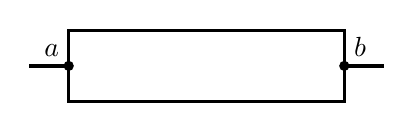
\begin{tikzpicture}[scale=.5]
        \draw[very thick](.5,.6) rectangle(7.5,2.4);
        \draw[very thick](-.5,1.5)--(.5,1.5);
        \draw[very thick](7.5,1.5)--(8.5,1.5);
        \fill(.5,1.5) circle(.13) node[above left] {$a$};
        \fill(7.5,1.5) circle(.13) node[above right]{$b$};
      \end{tikzpicture}

      Side View
      \vspace{.2in}
    \end{center}
    Explain your answer.
    \vspace{\stretch1}
    
    \part Calculate the strength of the electric field in the bar.
    \vspace{\stretch1}
    \newpage
    
    \uplevel{
      A uniform magnetic field of magnitude \SI{.25}{\tesla} perpendicular to
      the bar is added to the region around the bar, as shown below.
      \cpic{.8}{hall1}
    }

    \part Calculate the magnetic force on the bar.
    \vspace{\stretch1}
    
    \part The electrons moving through the bar are initially deflected by the
    external magnetic field. On the diagram below, indicate the direction of
    the additional electric field that is created in the bar by the deflected
    electrons.
    \begin{center}
      \vspace{.4in}
      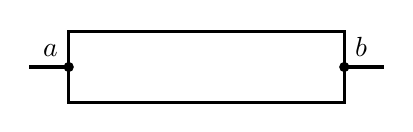
\begin{tikzpicture}[scale=.5, very thick]
        \draw (.5,.6) rectangle(7.5,2.4);
        \draw (-.5,1.5)--(.5,1.5);
        \draw (7.5,1.5)--(8.5,1.5);
        \fill(.5,1.5) circle(.13) node[above left] {$a$};
        \fill(7.5,1.5) circle(.13) node[above right]{$b$};
      \end{tikzpicture}

      Side View
      \vspace{.4in}
    \end{center}

    \part The electrons eventually experience no deflection and move through the
    bar at an average speed of \SI{3.5e-3}{\metre\per\second}. Calculate the
    strength of the additional electric field indicated in part (e).
    \vspace{\stretch2}        
  \end{parts}
  \newpage

  % TAKEN FROM THE 2009 AP PHYSICS C EXAM FREE-RESPONSE QUESTION E&M 3
  % THIS IS A QUESTION ON MAGNETIC INDUCTION
  \uplevel{
    \centering
    \begin{tikzpicture}[scale=.8]
      \foreach\x in {0,...,3}{
<<<<<<< HEAD
        \foreach\y in {0,...,3} \node[gray] at (\x,\y){$\bm\times$};
=======
        \foreach\y in {0,...,3} \node[black!70] at (\x,\y){$\bm\times$};
>>>>>>> 2022-09-fall
      }
      \draw[thick](-.5,-.5) to[rmeter,t=1](-.5,3.5)--(3.5,3.5)
      to[rmeter,t=2] (3.5,-.5)--(-.5,-.5);
      \node at (1.5,1.5){$B$};
      \draw[thick,|<->|](-.5,3.85)--(3.5,3.85) node[midway,fill=white]{$L$};
    \end{tikzpicture}
  }
  
  \question A square conducting loop of side $L$ contains two identical
  lightbulbs, 1 and 2, as shown above. There is a magnetic field directed into
  the page in the region inside the loop with magnitude as a function of time
  $t$ given by $B(t)=at+b$, where $a$ and $b$ are positive constants. The
  lightbulbs each have constant resistance $R_0$. Express all answers in terms
  of the given quantities and fundamental constants.
  \begin{parts}
    \part Derive an expression for the magnitude of the emf generated in the
    loop.
    \vspace{\stretch1}
    
    \part Determine an expression for the current through bulb 2.
    \vspace{\stretch1}

    \part Indicate on the diagram above the direction of the current through
    bulb 2.
    \vspace{\stretch1}
    
    \part Derive an expression for the power dissipated in bulb 1.
    \vspace{\stretch1}
    
    \uplevel{
      Another identical bulb 3 is now connected in parallel with bulb 2, but it
      is entirely outside the magnetic field, as shown below.
      \begin{center}
        \begin{tikzpicture}[scale=.8]
          \foreach\x in {0,...,3}{
<<<<<<< HEAD
            \foreach\y in {0,...,3} \node[gray] at (\x,\y){$\bm\times$};
=======
            \foreach\y in {0,...,3} \node[black!70] at (\x,\y){$\bm\times$};
>>>>>>> 2022-09-fall
          }
          \draw[thick](-.5,-.5) to[rmeter,t=1](-.5,3.5)--(3.5,3.5)
          to[rmeter,t=2] (3.5,-.5)--(-.5,-.5);
          \draw[thick](3.5,3.5)--(5.5,3.5) to[rmeter,t=3](5.5,-.5)--(3.5,-.5);
          \node at (1.5,1.5){$B$};
          \draw[thick,|<->|](-.5,3.85)--(3.5,3.85) node[midway,fill=white]{$L$};
        \end{tikzpicture}
      \end{center}
    }

    \part How does the brightness of bulb 1 compare to what it was in the
    previous circuit?

    \vspace{.1in}
    \underline{\hspace{.4in}} Brighter\hspace{.5in}
    \underline{\hspace{.4in}} Dimmer\hspace{.5in}
    \underline{\hspace{.4in}} The same

    \vspace{.1in}Justify your answer.
    \vspace{\stretch1}
    \newpage
    
    \uplevel{
      Now the portion of the circuit containing bulb 3 is removed, and a wire is
      added to connect the midpoints of the top and bottom of the original
      loop, as shown below.
      \begin{center}
        \begin{tikzpicture}[scale=.8]
          \foreach\x in {0,...,3}{
            \foreach\y in {0,...,3} \node[gray] at (\x,\y){$\bm\times$};
          }
          \draw[thick](-.5,-.5) to[rmeter,t=1](-.5,3.5)--(3.5,3.5)
          to[rmeter,t=2] (3.5,-.5)--(-.5,-.5);
          \draw[thick](1.5,3.5)--(1.5,-.5);
          \node at (.5,1.5){$B$};
          \node at (2.5,1.5){$B$};
          \draw[thick,|<->|](-.5,3.85)--(3.5,3.85) node[midway,fill=white]{$L$};
        \end{tikzpicture}
      \end{center}
    }

    \part How does the brightness of bulb 1 compare to what it was in the first
    circuit?

    \vspace{.1in}
    \underline{\hspace{.4in}} Brighter\hspace{.5in}
    \underline{\hspace{.4in}} Dimmer\hspace{.5in}
    \underline{\hspace{.4in}} The same
  \end{parts}

  \vspace{.1in}Justify your answer.
  \newpage

  \uplevel{
    \centering
    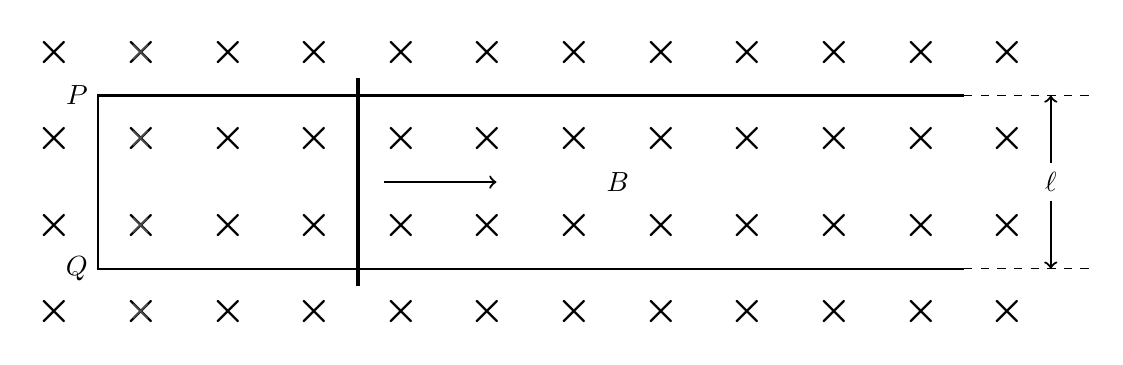
\begin{tikzpicture}[scale=1.1]
      \foreach \x in {0,...,11}
<<<<<<< HEAD
      \foreach \y in {0,...,3} \node at (\x,\y) {\Large$\bm\times$};
=======
      \foreach \y in {0,...,3} \node[black!70] at (\x,\y) {$\bm\times$};
>>>>>>> 2022-09-fall
      \draw[thick](10.5,.5)--(.5,.5) node[left]{$Q$}--(.5,2.5) node[left]{$P$}
      --(10.5,2.5);
      \draw[dashed](10.5,2.5)--(12,2.5);
      \draw[dashed](10.5,0.5)--(12,0.5);
      \draw[ultra thick](3.5,.3)--(3.5,2.7);
      \node at (6.5,1.5) {$B$};
      \draw[thick,<->](11.5,.5)--(11.5,2.5) node[midway,fill=white]{$\ell$};
      \draw[thick,->](3.8,1.5)--(5.1,1.5) node[midway,above]{$\varv$};
    \end{tikzpicture}

    Top View
  }
  
  \question In the diagram above, a nichrome wire of resistance per unit length
  $\lambda$ is bent at points $P$ and $Q$ to form horizontal conducting rails
  that are a distance $\ell$ apart. The wire is placed within a uniform
  magnetic field of magnitude $B$ pointing into the page. A conducting rod of
  negligible resistance, which was aligned with end $PQ$ at time $t=0$, slides
  to the right with constant speed $\varv$ and negligible friction. Express all
  algebraic answers in terms of the given quantities and fundamental constants.
  \begin{parts}
    \part Indicate the direction of the current induced in the circuit.

    \vspace{.1in}
    \underline{\hspace{.4in}} Clockwise\hspace{.5in}
    \underline{\hspace{.4in}} Counterclockwise

    \vspace{.1in}Justify your answer.
    \vspace{\stretch1}
    
`    \part Derive an expression for the magnitude of the induced current as a
    function of time $t$.
    \vspace{\stretch1}
    
    \part Derive an expression for the magnitude of the magnetic force on the
    rod as a function of time.
    \vspace{\stretch1}
    
    \part On the axes below, sketch a graph of the external force $F_\text{ext}$
    as a function of time that must be applied to the rod to keep it moving at
    constant speed while in the field. Label the values of any intercepts.
    \begin{center}
      \begin{tikzpicture}
        \draw[very thick,->](0,0)--(7,0) node[right]{$t$}
        node[pos=0,below left]{$O$};
        \draw[very thick,->](0,0)--(0,4) node[above]{$F_\text{ext}$};
      \end{tikzpicture}
    \end{center}
    \newpage
    
    \part The force pulling the rod is now removed. Indicate whether the speed
    of the rod increases, decreases, or remains the same.

    \vspace{.1in}
    \underline{\hspace{.4in}} Increases\hspace{.5in}
    \underline{\hspace{.4in}} Decreases\hspace{.5in}
    \underline{\hspace{.4in}} Remains the same
    
    \vspace{.1in}Justify your answer.
  \end{parts}

  \newpage

<<<<<<< HEAD
  % TAKEN FROM 2017 AP PHYSICS C FREE-RESPONSE QUESTION E&M 3
  \uplevel{
    \cpic{.7}{setup}
  }
  \question When studying Ampere's law, students collect data on the magnetic
  field of two different solenoids in order to determine the magnetic
  permeability of free space $\mu_0$. The solenoids are created by wrapping
  wire around a hollow plastic tube. The solenoids of length $\ell$ with $N$
  turns of wire will be connected in series to a power supply and resistor. A
  multimeter will be used as an ammeter to measure the magnitude of the current
  $I$ through the solenoids. The main components for the setup with one of the
  solenoids are shown in the figure above.
  \begin{parts}
    \part
    \begin{subparts}
      \subpart On the figure above, draw wire connections between the solenoid,
      power supply, resistor, and multimeter that will complete the circuit and
      allow students to measure the magnitude of the current through the
      solenoid.

      \subpart Using the connections you made in part (a)i above, what will be
      the direction of the magnetic field inside the solenoid?

      \vspace{.15in}
      \underline{\hspace{.6in}} Toward the top of the page\hspace{.5in}
      \underline{\hspace{.6in}} To the left\hspace{.5in}
      \underline{\hspace{.6in}} Out of the page\\
      \underline{\hspace{.6in}} Toward the bottom of the page\hspace{.26in}
      \underline{\hspace{.6in}} To the right\hspace{.42in}
      \underline{\hspace{.6in}} Into the page
      
      \uplevel{
        The rectangle shown below represents the solenoid (the loops of wire
        are not shown). Points $A$, $B$, and $C$ are along the central axis of
        the solenoid with point $B$ at the middle of the solenoid. Point $D$ is
        directly above point $B$.

        \vspace{.1in}
        \begin{center}
          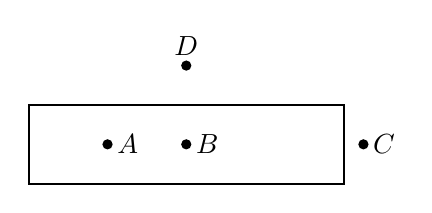
\begin{tikzpicture}
            \draw[thick] rectangle(4,1);
            \fill(1,.5) circle(.065) node[right]{$A$};
            \fill(2,.5) circle(.065) node[right]{$B$};
            \fill(4.25,.5) circle(.065) node[right]{$C$};
            \fill(2,1.5) circle(.065) node[above]{$D$};
          \end{tikzpicture}
        \end{center}
        \vspace{.15in}
      }
      
      \subpart From the choices below, select the point where you would place a
      magnetic field probe (a probe that can measure the magnitude of the
      magnetic field) to best measure the strength of the magnetic field of the
      solenoid in order to determine the magnetic permeability of free space
      $\mu_0$. Justify your answer based on the model for a simple solenoid.

      \vspace{.15in}
      \underline{\hspace{.5in}} A\hspace{.5in}
      \underline{\hspace{.5in}} B\hspace{.5in}
      \underline{\hspace{.5in}} C\hspace{.5in}
      \underline{\hspace{.5in}} D
    \end{subparts}
    \newpage
    
    \uplevel{
      The figures below show two different solenoids that will be connected in
      the circuit above. Solenoid 1 has a length $\ell=\SI{25}{\centi\metre}$
      with $N=100$ turns. Solenoid 2 has a length $\ell=\SI{5.}{\centi\metre}$
      with $N=5$ turns.
      \begin{center}
        \pic{.5}{2solenoids}
        
        \underline{Note:} Figures not drawn to scale.
      \end{center}

      \vspace{.1in}A graph of the magnitude of the magnetic field $B$ as a
      function of $NI/\ell$ is shown below. The best-fit lines for the data are
      shown as a solid line for solenoid 1 and as a dashed line for solenoid 2.

      \cpic{.7}{results}
    }

    \part Which solenoid's best-fit line would give the best results for
    determining a value for the magnetic permeability of free space $\mu_0$?
    Justify your answer.
    
    \vspace{.1in}
    \underline{\hspace{.5in}} Solenoid 1\hspace{.5in}
    \underline{\hspace{.5in}} Solenoid 2

    \part
    \begin{subparts}
      \subpart Use the slope of the best-fit line for the solenoid chosen in
      part (b) to calculate the magnetic permeability of free space $\mu_0$.

      \subpart Calculate the percent error for the experimental value of the
      magnetic permeability of free space $\mu_0$ determined in part (c)i.
    \end{subparts}

    \part
    \begin{subparts}
      \subpart What is a reasonable physical explanation for a best-fit line
      that does not pass through the origin?

      \subpart Suppose a student connects the solenoid in a closed circuit
      similar to the circuit in part (a)i but without the resistor. The student
      notices the multimeter stops functioning after the power supply is turned
      on. Explain what causes the failure of the multimeter.
    \end{subparts}
  \end{parts}
=======
%  % TAKEN FROM 2017 AP PHYSICS C FREE-RESPONSE QUESTION E&M 3
%  \uplevel{
%    \cpic{.7}{setup}
%  }
%  \question When studying Ampere's law, students collect data on the magnetic
%  field of two different solenoids in order to determine the magnetic
%  permeability of free space $\mu_0$. The solenoids are created by wrapping
%  wire around a hollow plastic tube. The solenoids of length $\ell$ with $N$
%  turns of wire will be connected in series to a power supply and resistor. A
%  multimeter will be used as an ammeter to measure the magnitude of the current
%  $I$ through the solenoids. The main components for the setup with one of the
%  solenoids are shown in the figure above.
%  \begin{parts}
%    \part
%    \begin{subparts}
%      \subpart On the figure above, draw wire connections between the solenoid,
%      power supply, resistor, and multimeter that will complete the circuit and
%      allow students to measure the magnitude of the current through the
%      solenoid.
%
%      \subpart Using the connections you made in part (a)i above, what will be
%      the direction of the magnetic field inside the solenoid?
%
%      \vspace{.15in}
%      \underline{\hspace{.6in}} Toward the top of the page\hspace{.5in}
%      \underline{\hspace{.6in}} To the left\hspace{.5in}
%      \underline{\hspace{.6in}} Out of the page\\
%      \underline{\hspace{.6in}} Toward the bottom of the page\hspace{.26in}
%      \underline{\hspace{.6in}} To the right\hspace{.42in}
%      \underline{\hspace{.6in}} Into the page
%      
%      \uplevel{
%        The rectangle shown below represents the solenoid (the loops of wire
%        are not shown). Points $A$, $B$, and $C$ are along the central axis of
%        the solenoid with point $B$ at the middle of the solenoid. Point $D$ is
%        directly above point $B$.
%
%        \vspace{.1in}
%        \begin{center}
%          \begin{tikzpicture}
%            \draw[thick] rectangle(4,1);
%            \fill(1,.5) circle(.065) node[right]{$A$};
%            \fill(2,.5) circle(.065) node[right]{$B$};
%            \fill(4.25,.5) circle(.065) node[right]{$C$};
%            \fill(2,1.5) circle(.065) node[above]{$D$};
%          \end{tikzpicture}
%        \end{center}
%        \vspace{.15in}
%      }
%      
%      \subpart From the choices below, select the point where you would place a
%      magnetic field probe (a probe that can measure the magnitude of the
%      magnetic field) to best measure the strength of the magnetic field of the
%      solenoid in order to determine the magnetic permeability of free space
%      $\mu_0$. Justify your answer based on the model for a simple solenoid.
%
%      \vspace{.15in}
%      \underline{\hspace{.5in}} A\hspace{.5in}
%      \underline{\hspace{.5in}} B\hspace{.5in}
%      \underline{\hspace{.5in}} C\hspace{.5in}
%      \underline{\hspace{.5in}} D
%    \end{subparts}
%    \newpage
%    
%    \uplevel{
%      The figures below show two different solenoids that will be connected in
%      the circuit above. Solenoid 1 has a length $\ell=\SI{25}{\centi\metre}$
%      with $N=100$ turns. Solenoid 2 has a length $\ell=\SI{5.}{\centi\metre}$
%      with $N=5$ turns.
%      \begin{center}
%        \pic{.5}{2solenoids}
%        
%        \underline{Note:} Figures not drawn to scale.
%      \end{center}
%
%      \vspace{.1in}A graph of the magnitude of the magnetic field $B$ as a
%      function of $NI/\ell$ is shown below. The best-fit lines for the data are
%      shown as a solid line for solenoid 1 and as a dashed line for solenoid 2.
%
%      \cpic{.7}{results}
%    }
%
%    \part Which solenoid's best-fit line would give the best results for
%    determining a value for the magnetic permeability of free space $\mu_0$?
%    Justify your answer.
%    
%    \vspace{.1in}
%    \underline{\hspace{.5in}} Solenoid 1\hspace{.5in}
%    \underline{\hspace{.5in}} Solenoid 2
%
%    \part
%    \begin{subparts}
%      \subpart Use the slope of the best-fit line for the solenoid chosen in
%      part (b) to calculate the magnetic permeability of free space $\mu_o$.
%
%      \subpart Calculate the percent error for the experimental value of the
%      magnetic permeability of free space $\mu_0$ determined in part (c)i.
%    \end{subparts}
%
%    \part
%    \begin{subparts}
%      \subpart What is a reasonable physical explanation for a best-fit line
%      that does not pass through the origin?
%
%      \subpart Suppose a student connects the solenoid in a closed circuit
%      similar to the circuit in part (a)i but without the resistor. The student
%      notices the multimeter stops functioning after the power supply is turned
%      on. Explain what causes the failure of the multimeter.
%    \end{subparts}
%  \end{parts}
>>>>>>> 2022-09-fall
\end{questions}
\end{document}
